\documentclass{article}
\usepackage{fullpage}
\usepackage{amsmath, amssymb}
\usepackage[hidelinks]{hyperref}
\usepackage{natbib}
\usepackage{xcolor}
\usepackage{graphics}

\newcommand{\E}{\mathbb{E}}
\renewcommand{\P}{\mathbb{P}}

\newcommand{\comment}[1]{{\color{blue} \it #1}}

\begin{document}

% 1. *Intro*: Motivation about how many results about quant gen and methods assume Gaussian distributions.
%     Mention Levy walk macroevolution papers.
%     Point out that usual quant gen has *no* sweeps, while stable distributions would have sweeps (since some s would be bigger than 1/N).
%     Motivate with mixture model of effect sizes.
%     If stable distributions are a better model, what does that tell us? We can better understand the *noise* in evolution, i.e., predictability and saltation-ness.
%     (PETER)
% 
% 2. Motivation: empirical SNPs distributions in real data (PETER)
% 
% 3. Introducing infinitesimal model (in this case) (TODD)
% 
% 4. Proof following BEV in stable case (TODD)
% 
% 5. Theoretical results on stationary distributions (TODD)
% 
% 6. Simulations (PETER)

\title{\large{\bf
    Quantitative genetics with stable laws
}}

\author{ \begin{small}
    Todd Parsons \&
    Peter Ralph
\end{small}}

\date{\today}
\maketitle

\begin{abstract}
\end{abstract}

%%%%%%%%%%%%%%%%%%%%%%
\section{Introduction}

Much of the work to give a quantitative understanding to the observation that
offspring of sexual organisms resemble their parent,
has focused on \emph{quantitative genetics},
which is interestingly intermediate between a mechanistic model of genetics
and a purely phenomenological model.
The action of natural selection on genetic variants in the absence of genetic variation
is relatively well-understood (cite ewens),
but tractable mathematical models of evolution for recombining species
are elusive,
at least with some results of when the model might be a good description of reality.
For instance, a great deal of conceptual understanding and even quantitative predictions
have been made assuming that the distribution of trait values in a population is Gaussian
(cite Lande etcetera)
despite the absence of a plausible model that would make this true (cite turelli and barton).
One of the oldest and most concrete models of heritable trait evolution is the \emph{infinitesimal model}
which assumes a simple, explicit form for how an offspring's trait is inherited from their parents':
it is Normally distributed, with mean equal to the average of the parents' values.
Despite the inherent plausibility of this model,
(thanks to the Central Limit Theorem),
it was not until \citet{barton2017infinitesimal} that conditions under which this would be a good approximation
were made explicit,
through a formal convergence proof.

As suggested by its name, under the infinitesimal model the effects of any given genetic variant on the trait
is small (indeed, vanishing),
and so selection-driven trait shifts are mediated by small changes in frequencies of many alleles of small effect.
However, empirical understanding of the genetic basis of trait variation in real-world species
often finds a significant portion of heritable variation explained by variants at only a few loci.
There are many possible explanations for this observation,
including selection/publication bias,
filters for larger-effect variants due to spatially varying selection (cite),
ond/or grouping together of concordant alleles by linkage or inversions (cite).
However, it seems clear that in at least those cases where we understand the underlying molecular mechanisms
that mutations of large effect can be important in practice
(cite examples: insecticide resistance, coloration, etc),
and the consensus in the field is that traits exist on a spectrum between monogenic and polygenic,
and that many - if not most - are firmly in the intermediate, ``oligogenic'' region (cite),
where heritable trait variation is due both to segregating large- and small-effect variants.
Indeed, some sensible verbal models of the biological mechanisms by which a genetic change
comes to have an effect on an organism's trait
describe a hierarchy or range of ``proximities'' to the trait,
by which changes to more ``nearby'' genes have the possibility of causing larger changes in the trait
(cite omnigenic and others).
This suggests a mixture model for the effect size distribution:
perhaps the distribution of effect sizes within each gene is Normal,
but with a standard deviation that varies with ``proximity'' to the trait;
such mixtures can easily have large proportions of extreme values.

The infinitesimal model gains a great deal of generality by appealing to the Central Limit Theorem:
as shown by \citet{barton2017infinitesimal},
the distribution of segregation noise will be Normal, regardless of most of the details,
thanks to the universality of adding up a great many very small and independent things.
However, as is well known to probabilists,
there is a wider class of Central Limit Theorems,
which describe the distributions of sums of a great many independent and exchangeable things:
the \emph{stable laws}.
Roughly speaking, these say that if we add together $n$ independent copies of a random variable $X$
for which $\P\{ X > t \} \propto t^{-\alpha}$ for some $0 < \alpha < 2$,
then -- almost regardless of the details -- the result, scaled by $n^{1/\alpha}$,
is well-approximated by a universal form, the $\alpha$-stable distribution (and becomes exact, as $n \to \infty$).
In such ensembles, sinle large entries are important:
concretely, the largest of the $n$ copies will be of order $n^{1/\alpha}$,
so that e.g., for $\alpha=1$ a positive proportion of the sum of $n$ entries will be contributed by a single one.

This suggests exploring whether stable distributions might reasonably stand in for the Normal
in the infinitesimal model.
In this paper, we make rather preliminary explorations in that direction:
Does the universality shown by \citet{barton2017infinitesimal}
carry over when the distribution of effect sizes falls in the domain of attraction of a stable law?
What can be said about equilibrium trait distributions in this case?
And, is there any biological evidence that this theory might be relevant?

Stable distributions are by no means new to population biology.
For instance, it is a long-standing question how often the motions of organisms
are better modeled by essentially Brownian random walks or by L\'evy processes (cite),
and a growing literature studies the effects of such ``fat-tailed'' distributions
on the shapes and dynamics of traveling waves such as biological invasions (cite).
\comment{Other examples?}
More directly analogous to the problem we study here, \citet{landis2012phylogenetic}
found that an $\alpha$-stable process (with $\alpha \approx 1.5$) fit the evolution of log endocranial volume
on the primate phylogeny
better than either a Brownian model.
\comment{more}

\comment{TODO expand, put somewhere:}
There are several justifications for why a ``stable infinitesimal model'' might be useful:
(1) as a phenomenological model;
(2) if it matches empirical observations; or
(3) if there is a central limit theorem suggesting it would be a good approximation in a wide range of situations.

\subsection*{Orphaned text}
The ways in which genetic variants combine to determine an organisms' trait can be complex,
and epistatic interactions between alleles and between loci can be important in practice.
However, the question is sufficiently complex in the purely additive case
that a trait can be decomposed into a sum across loci of the contributions of the alleles from each locus.
Under this additive assumption it makes sense to discuss the ``effect size distribution'',
i.e., the distribution of how much alleles affect the trait value.

An offspring's trait differs from their parents for many reasons,
often most importantly because of differences in the environment in which they live.
The focus of quantitative genetics is on the contribution of heritable material to this variation:
the offspring's genetic material 


\comment{Will need this notation below:}
We focus on the \emph{infinitesimal model},
as described by \citet{barton2017infinitesimal},
which supposes that the trait value of an offspring
is equal to the average of their parents' trait values,
plus independent Gaussian noise with fixed variance,
\begin{equation} \label{eqn:offspring_model}
    X_o = \frac{X_m + X_f}{2} + \epsilon,
\end{equation}
where $\epsilon$, the ``segregation noise'',
is Gaussian with mean zero and variance $V_0$.
\comment{should call this something besides $\epsilon$}

%%%%%%%%%%%%%%%%%%%%%%
\section{Empirical observations}

It is mathematically intriguing to speculate what effect a non-Gaussian distribution
for $\epsilon$ would have on the dynamics induced by~\eqref{eqn:offspring_model}.
But, is there any evidence that non-Gaussian segregation noise is important in practice?
In this paper we focus primarily on the theory,
but first take a brief and imperfect look at what some data have to say on the topic.
To do this, we downloaded the GWAS results provided by~\citet{biobankSNPs}
for 7,221 phenotypes from 361,194 individuals from the March 2018 release of the UK Biobank.
After filtering (see details below) we were left with 695 binary illness-related phenotypes.
Taken at face value, these provide for each phenotype a set of estimates of the additive effect
of the alternative allele at a set of SNPs on the phenotype relative to the reference allele.
The phenotypes we consider were all binary and coded as 0/1,
so estimates could be thought of as additive adjustments to the risk
(i.e., effects are \emph{not} on a logit scale).
These estimates were obtained as the coefficient for the SNP in a simple linear model
fit to each phenotype for each SNP,
with the first 20 principal components and all combinations of age, age squared, and inferred sex as covariates;
we considered effects of those SNPs with a reported $p$-value less than $10^{-8}$.
There are a great many possible issues with these data;
however, the results seem consistent across many SNPs and phenotypes,
and we know of no reason that possible methodological artifacts
(e.g., confounding by uncorrected variables)
would specifically affect the decay of the tail of effect sizes.

Suppose that the phenotype of each individual is additive:
the maternal trait value is $x = \sum_i x_{i,1} + x_{i,2}$
and the paternal trait value is $y = \sum_i y_{i,1} + y_{i,2}$,
where $x_{i,1}$ and $x_{i,2}$ are the effects of the alleles carried
by the mother on each of the two chromosomes
at the $i^\text{th}$ locus, respectively.
Then the offspring's trait is $z = \sum_i z_{i,m} + z_{i,p}$,
where $z_{i,m} = \theta_{i,m} x_{i,1} + (1-\theta_{i,m}) x_{i,2}$,
and $\theta_{i,m} = 1$ with probability 1/2 and $\theta_{i,m} = 0$ otherwise;
and likewise $z_{i,p} = \theta_{i,p} y_{i,1} + (1-\theta_{i,p}) y_{i,2}$.
With this notation, the segregation noise $z - \frac{x+y}{2}$
is a sum of terms of the form
$$
    \left( \theta_{i,m} - 1/2 \right) x_{i,1}
    + \left( 1/2 - \theta_{i,m} \right) x_{i,2} 
$$
(and similar terms with $y$ in place of $x$).
Now let $X$ be the effect of a uniformly chosen allele carried by a uniformly chosen individual
at a uniformly chosen locus.
The appropriate central limit theorem is determined by the tail behavior of $|(\theta - 1/2) X| = |X|/2$.
So, we'd like to know the value of
$$
    \lim_{t \to \infty} \frac{ \log \P\{ |X| > 2 t \} }{ \log t } = \alpha ,
$$
if the limit exists.
Let $p_i$ be the minor allele frequency at the $i^\text{th}$ locus;
since the data we have assigns effect 0 to the major allele,
$x_i = 0$ with probability $1-p_i$.
Therefore, if we have estimated effects for $N$ SNPs
with minor allele frequency $p_i$ and effect size $e_i$ for the minor allele,
for $1 \le i \le N$,
then
$$
    \P\{ |X| > 2t \} \approx \frac{1}{N} \sum_{i : |e_i| > 2t} p_i .
$$
So, to obtain a per-trait estimate of $\alpha$,
we plot $\log \frac{1}{N} \sum_{i : |e_i| > t} p_i$ against $\log t$
for a sequence of values of $t$,
and fit a linear model to the tail
(which we take to be all values of $t$ for which the number of SNPs with absolute effect above $t$
is between 20 and 10\% of all SNPs).
Examples are shown in figure~\ref{fig:example_snps}.

\begin{figure}
    \begin{center}
    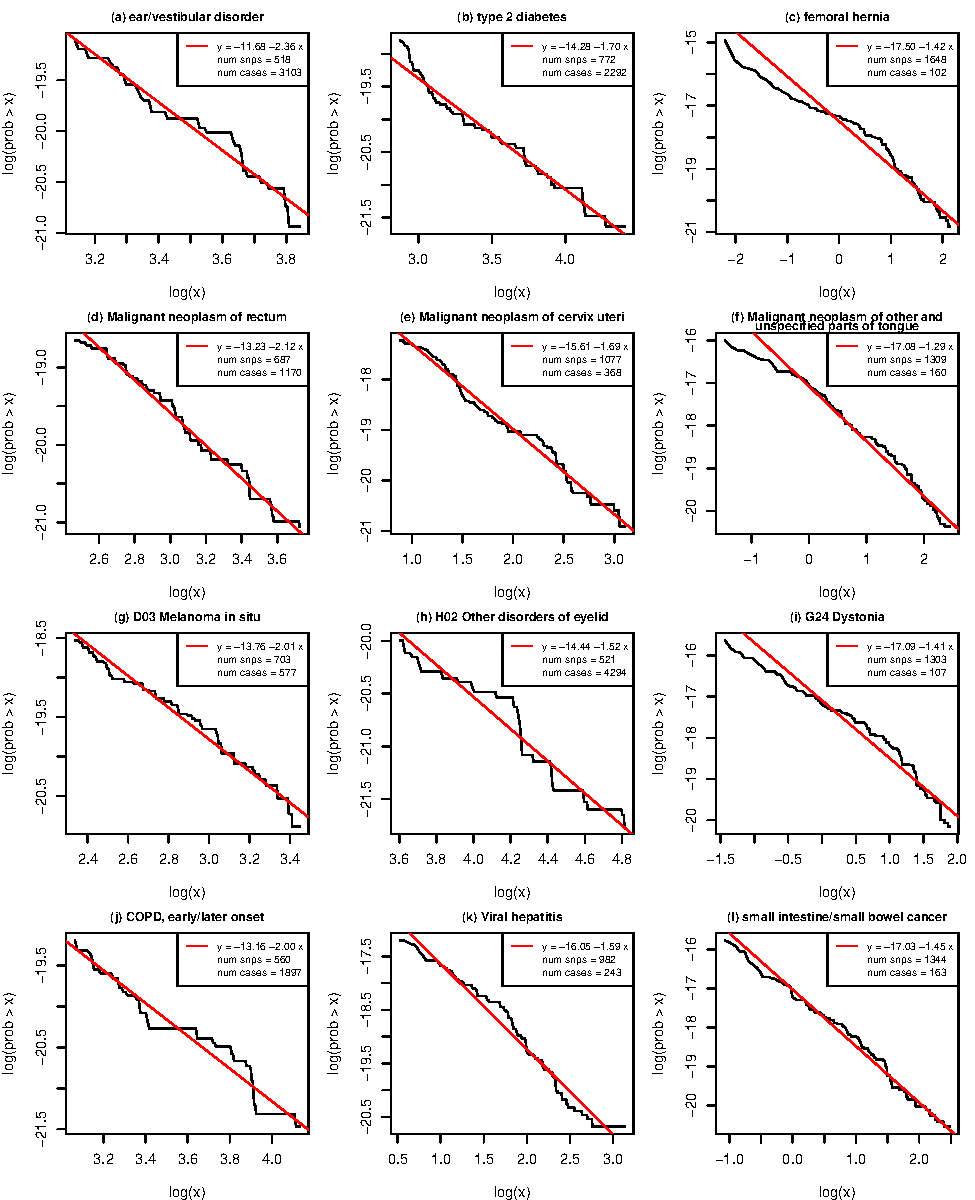
\includegraphics{snp_effects/examples}
    \end{center}
    \caption{
        TODO: cut this down to just 2 SNPs and move this figure to the supplement; change 'x' to 't' in axis labels.
        Tail distributions of frequency-weighted effects
        for twelve randomly chosen phenotypes.
        In each, for a phenotype with $N$ SNPs,
        effect sizes $e_i$ and frequencies $p_i$,
        the black line shows
        $\log \frac{1}{N} \sum_{i : |e_i| > t} p_i$ (vertical axis)
        against $\log t$ (horizontal axis);
        the red line shows the least-squares linear fit;
        each plot only covers the 10\% largest-effect SNPs.
        Legends show the coefficients of the red line; the slope on `x' is $\alpha$,
        the estimated exponent;
        ``num snps'' is the number of SNPs for the phenotype with $p$-value less than $10^{-8}$,
        and ``num cases'' is the reported number of the rougly 360,000 individuals
        recorded as having the listed phenotype.
        \label{fig:example_snps}
    }
\end{figure}

We applied this procedure to results from models fit on both sexes,
after removed phenotypes related to employment, drug treatments, and diet.
This left us with 1,108 phenotypes for which which could estimate the tail exponent.
For the main results,
we then restricted to phenotypes having non-missing numbers of ``cases'' and ``controls''
and a sample size of at least 300,000 (i.e., not more than 61,194 of 361,194 missing phenotypes).
We also removed
the 65 remaining phenotypes that are common (more than 10,000 cases),
as these often showed very different patterns
(e.g., effect size distributions).
This left us with 695 phenotypes;
plots including the 413 ``filtered'' phenotypes are provided in
Supplementary Figure~\ref{sfig:unfiltered_hist}.

Resulting values of the tail exponent $\alpha$ are shown in Figure~\ref{fig:exponent_hist}.
Estimated tail exponents range from about 1 to 2.5,
and 28.9\% had estimated values less than 1.5.
A concern could be that ``noisier'' phenotypes,
for which estimated effect sizes are less reliable,
might lead to larger estimated tail exponents;
for this reasons, we looked for an association between
tail exponent and two proxies for power,
number of SNPs (i.e., number of SNPs with $p$-value less than $10^{-8}$)
and number of cases.
Interestingly, the result in nonmonotonic,
with exponents closer to $\alpha=2$ for phenotypes with around 1000 cases,
and lower exponents for rarer \emph{and} more common phenotypes.
(A similar pattern is seen for ``number of SNPs'',
but this may be due to association with number of cases.)
This may indicate a statistical artifact,
or it may be a result of biological differences in genetic architecture
between more and less common phenotypes.

\begin{figure}
    \begin{center}
    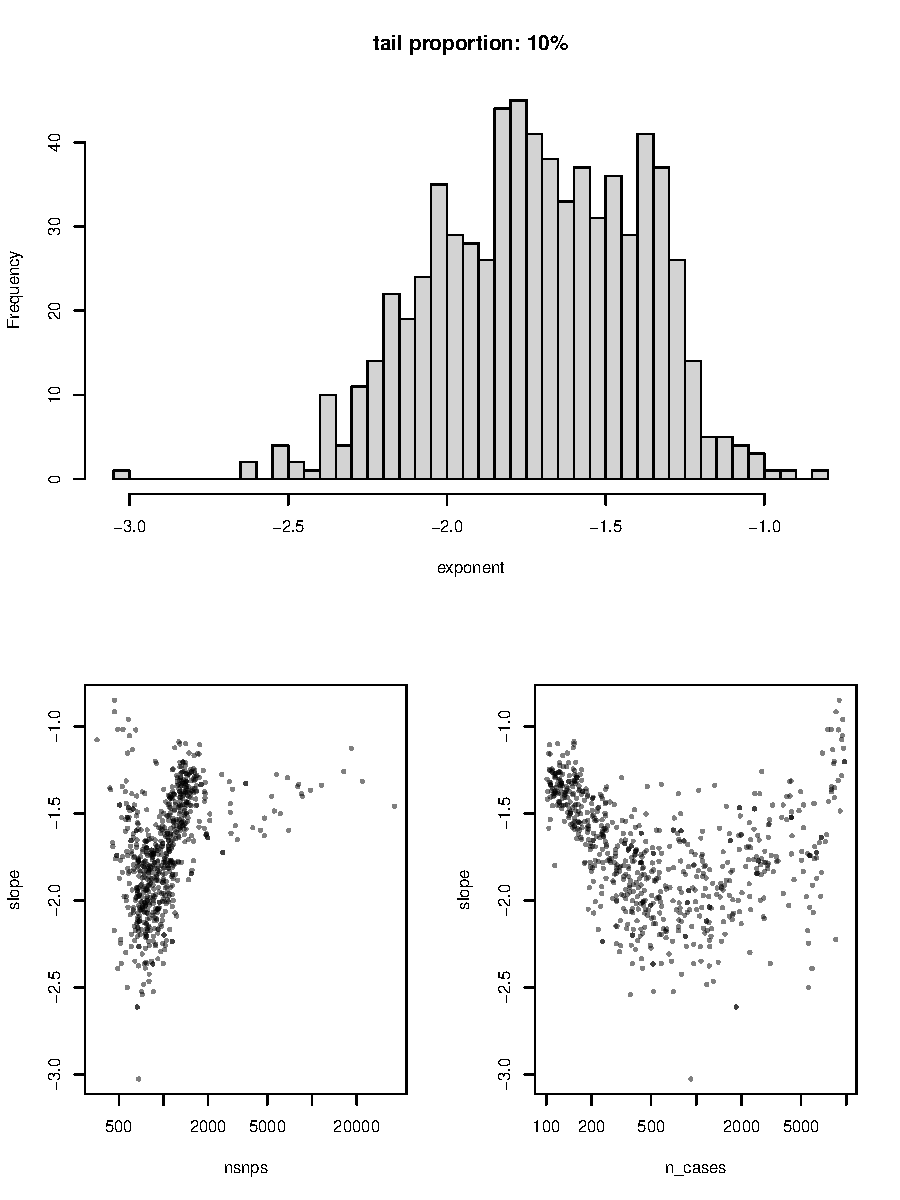
\includegraphics{snp_effects/results_10}
    \end{center}
    \caption{
        Estimated values of the tail exponent, $\alpha$,
        for 775 illness-related binary phenotypes:
        \textbf{(A)} distribution of values; and plotted against
        \textbf{(B)} number of SNPs, and
        \textbf{(C)} number of cases.
        \label{fig:exponent_hist}
    }
\end{figure}


%%%%%%%%%%%%%%%%%%%%%%
\section{Extending the infinitesimal model}  % TODD

%%%%%%%%%%%%%%%%%%%%%%
\section{Convergence to the non-infinitesimal model}  % TODD

%%%%%%%%%%%%%%%%%%%%%%
\section{Stationary distributions}  % TODD

%%%%%%%%%%%%%%%%%%%%%%
\section{Simulations}  % PETER


\bibliographystyle{plainnat}
\bibliography{refs}

\appendix

\begin{figure}
    \begin{center}
    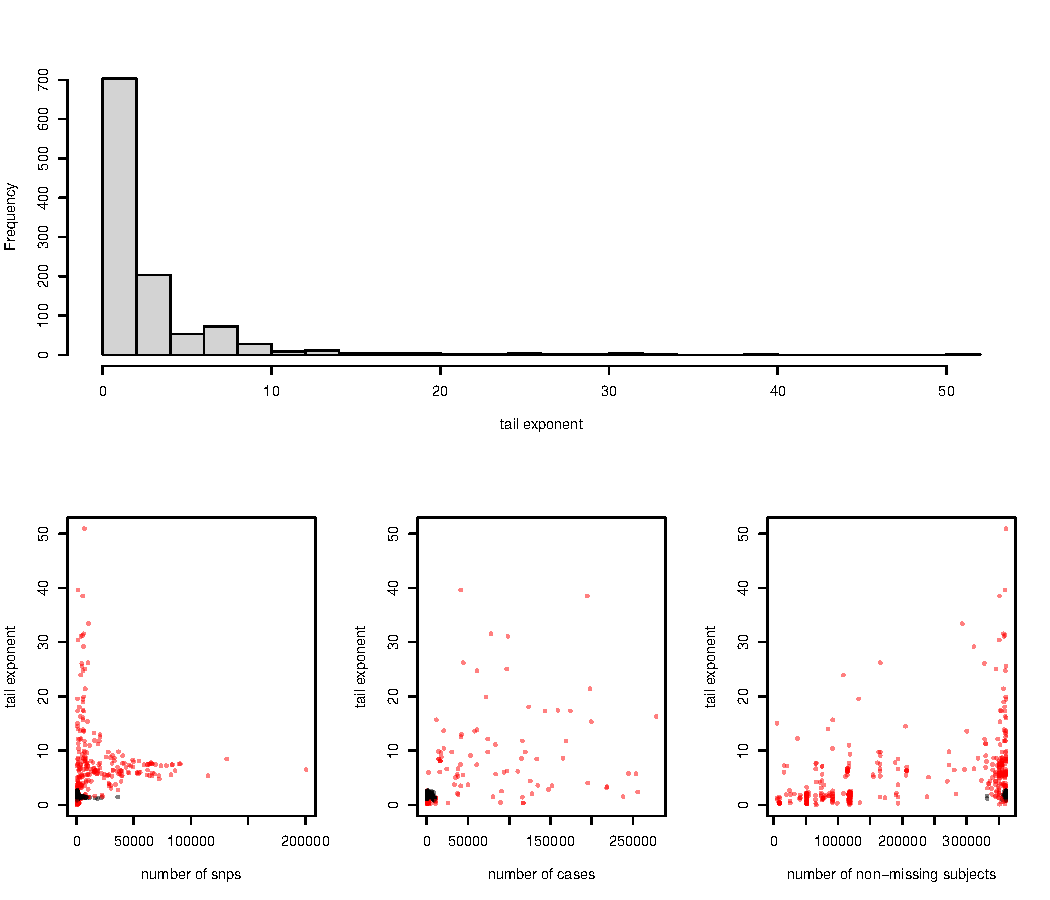
\includegraphics{snp_effects/unfiltered_results_10}
    \end{center}
    \caption{
        Estimated values of the tail exponent, $\alpha$,
        for 1108 illness-related binary phenotypes,
        including the 333 phenotypes removed in filtering,
        which are shown as red points in lower plots.
        \textbf{(A)} distribution of values; and plotted against
        \textbf{(B)} number of SNPs,
        \textbf{(C)} number of cases, and
        \textbf{(C)} number of non-missing subjects.
        \label{fig:unfiltered_hist}
    }
\end{figure}

\end{document}
